

\subsection{GIA Calculation Results}



Listed in this section are the results of each of the possible combinations of sites.
Since 4 sites were used, a total of 6 distinct combinations of sites were studied.


\begin{figure}[h]
	\makebox[\textwidth]{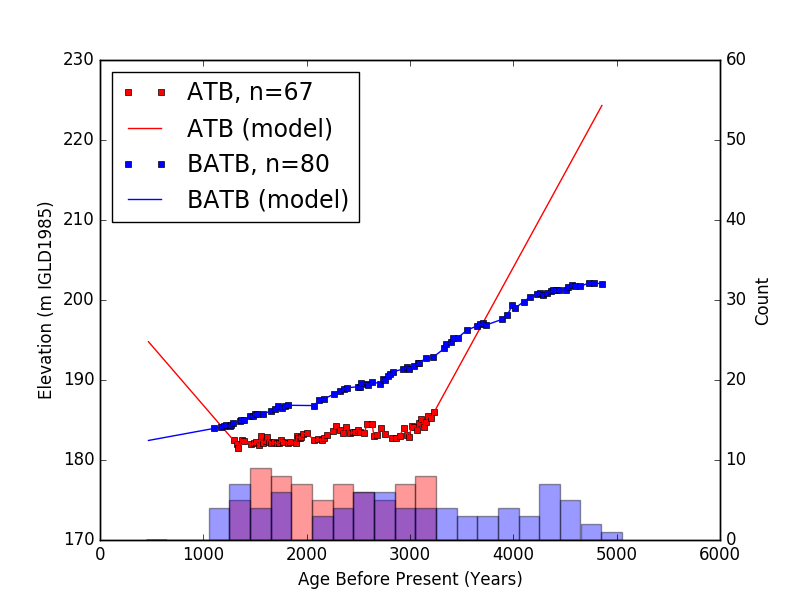
\includegraphics[width=0.72\paperwidth]{data/ATB-BATB_DataAndModel.png}}
	\caption{Measured and modelled elevation data plotted against age for sites ATB \& BATB}
	\label{fig:data_ATBxBATB}
\end{figure}
The data available for sites ATB and BATB shows two of the most common trends in
 the data used in this paper; Data is available for both sites from
 approximately 1000 years before present to roughly 3300 years before present,
 with a gap in the record at around 2000 years before present (caused by a low
 water level period preferentially not forming beach deposits during this time)
 (Johnston et al, 2014). With the data divided up into bins of 200 years width
 starting at 1050 years before present, the data from every bin between 1250 and 3250 was used
 in calculating a rate of gia, save for the previously mentioned gap from 1850-2050
 years before present (where comparisons between data in the ATB dataset would be
 subtracting against a modelled value for BATB that is likely unreliable given
 the distance to the nearest datapoint in BATB). The regressions derived from this pair of data sets,
 seen in Figures \ref{fig:gias_ATBxBATB} \& \ref{fig:gias_BATBxATB}, are well
 constrained, and produce a moderately well constrained value on relative GIA
 between ATB and BATB of 23.5-31 cm/century. A plot of the confidence intervals
 for the slopes obtained from each linear regression can be seen in Figure \ref{fig:intervalsGIA}


\newpage

\begin{figure}[h]
	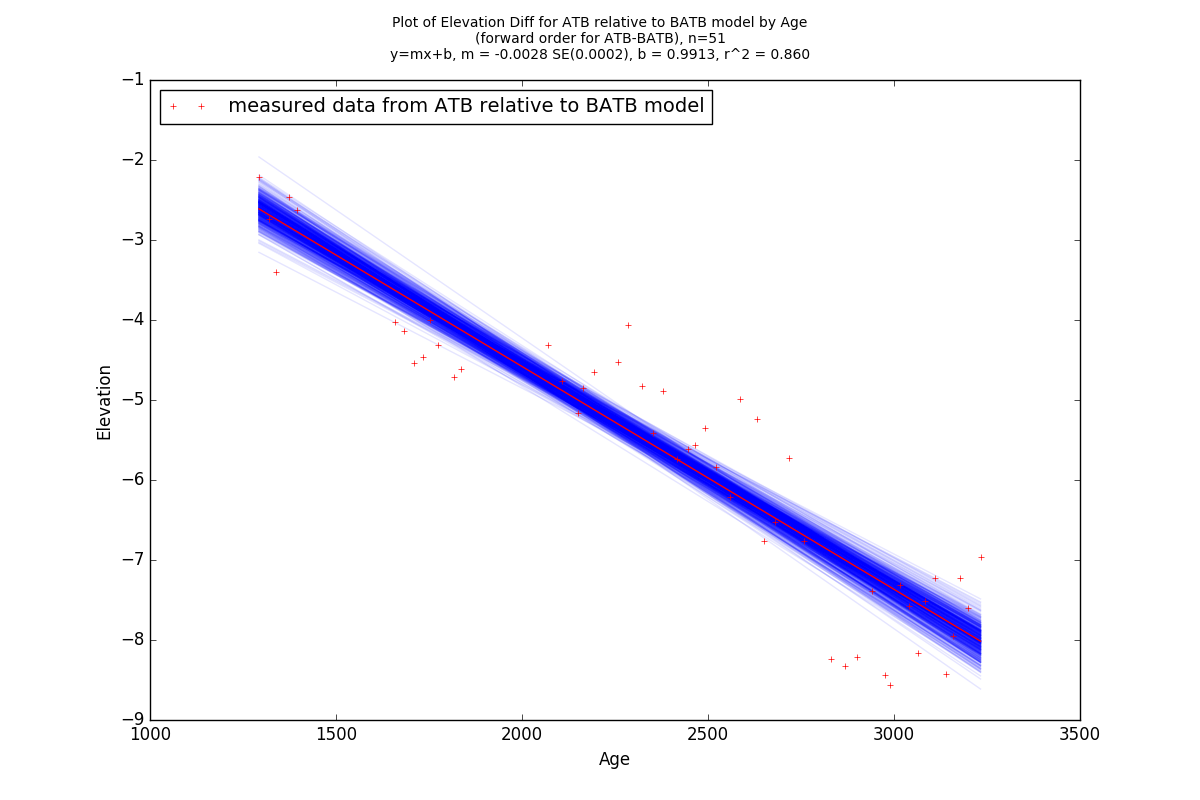
\includegraphics[width=0.9\linewidth]{data/bothNonZero/withinSeventyFivePercent/gias/theGIA_ATB_relative_to_BATB.png}
	\caption{Differences in elevation measured from the ATB data to the ATB model}
	\label{fig:gias_ATBxBATB}
\end{figure}
\newpage


\begin{figure}[h]
	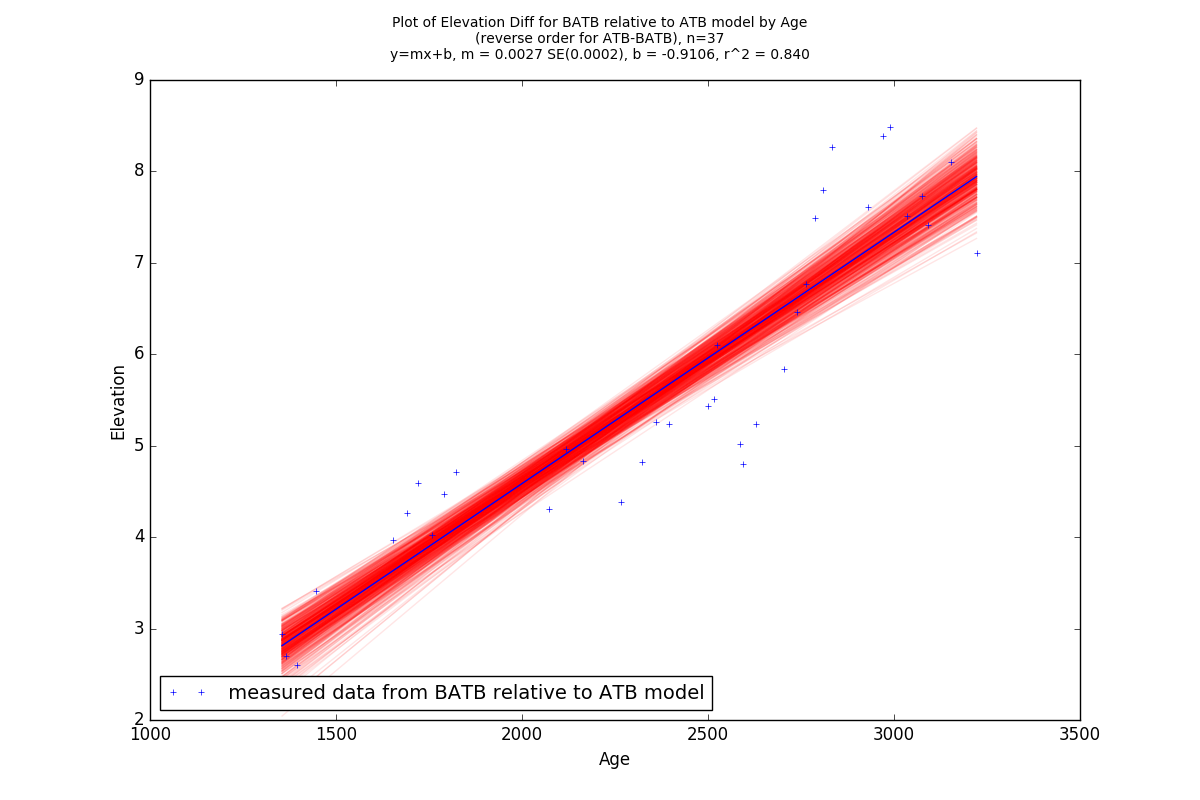
\includegraphics[width=0.9\linewidth]{data/bothNonZero/withinSeventyFivePercent/gias/theGIA_BATB_relative_to_ATB.png}
	\caption{Differences in elevation measured from the BATB data to the ATB model}
	\label{fig:gias_BATBxATB}
\end{figure}
\newpage
% this desperately needs to be done as a loop



\begin{figure}[h]
	\makebox[\textwidth]{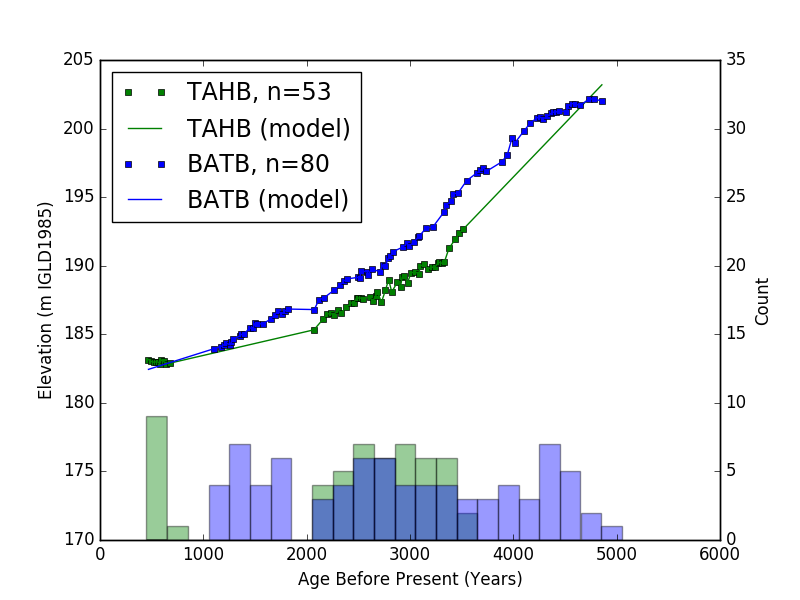
\includegraphics[width=0.72\paperwidth]{data/TAHB-BATB_DataAndModel.png}}
	\caption{TAHB-BATB raw data with linear interpolation model}
	\label{fig:data_TAHBxBATB}
\end{figure}

The data plot for the site combination of TAHB and BATB shows a common issue
with comparing datasets, as the data with ages more recent than the 2000 year before
present gap is unsable. This is because the regions where data is available for
one dataset are empty of datapoints for the other, making the modelled prediction
of the other dataset highly unreliable. As a result, a filter is applied to the
data to prevent this, grouping data points into bins 200 years wide, and
ignoring the data points from bins in which either data set had no datapoints,
as well as any which had bin counts differing by more than 75\% for that bin.
As a result, only the data from 2050 to 3650 years before present were used in
creating the GIA comparisons.\\
The linear regressions produced from this dataset seen in Figures 
\ref{fig:gias_TAHBxBATB} \& \ref{fig:gias_BATBxTAHB}, are well constrained, and
report a value for relative GIA of between 11-16.7 cm/century.

\newpage

\begin{figure}[h]
	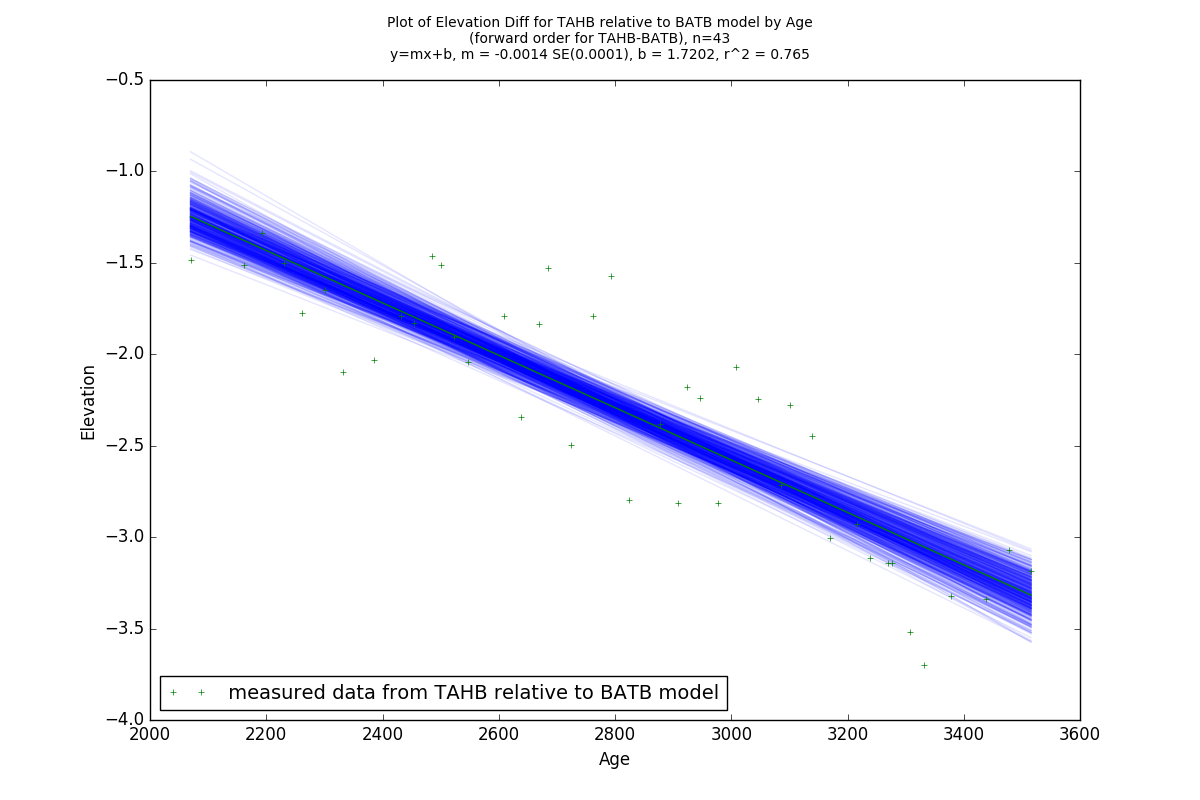
\includegraphics[width=0.9\linewidth]{data/bothNonZero/withinSeventyFivePercent/gias/theGIA_TAHB_relative_to_BATB.png}
	\caption{Differences in elevation measured from the TAHB data to the BATB model}
	\label{fig:gias_TAHBxBATB}
\end{figure}
\newpage


\begin{figure}[h]
	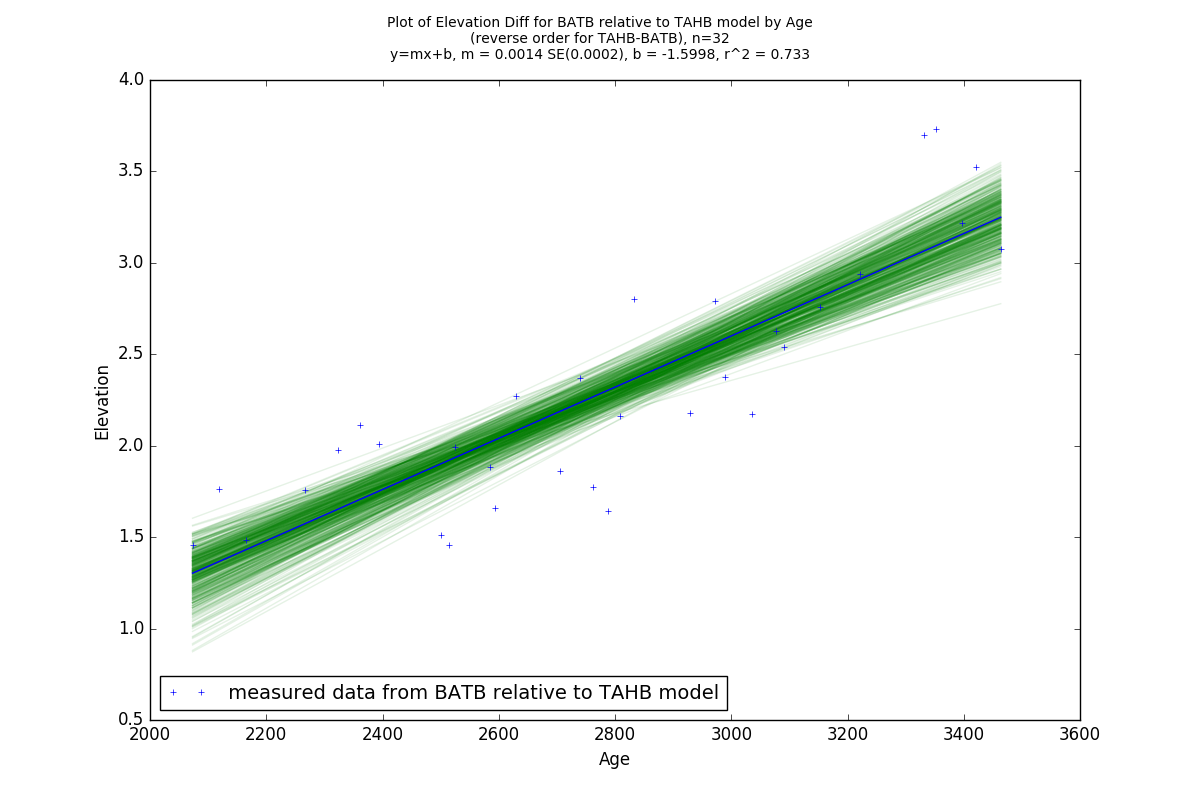
\includegraphics[width=0.9\linewidth]{data/bothNonZero/withinSeventyFivePercent/gias/theGIA_BATB_relative_to_TAHB.png}
	\caption{Differences in elevation measured from the BATB data to the TAHB model}
	\label{fig:gias_BATBxTAHB}
\end{figure}
\newpage








\begin{figure}[h]
	\makebox[\textwidth]{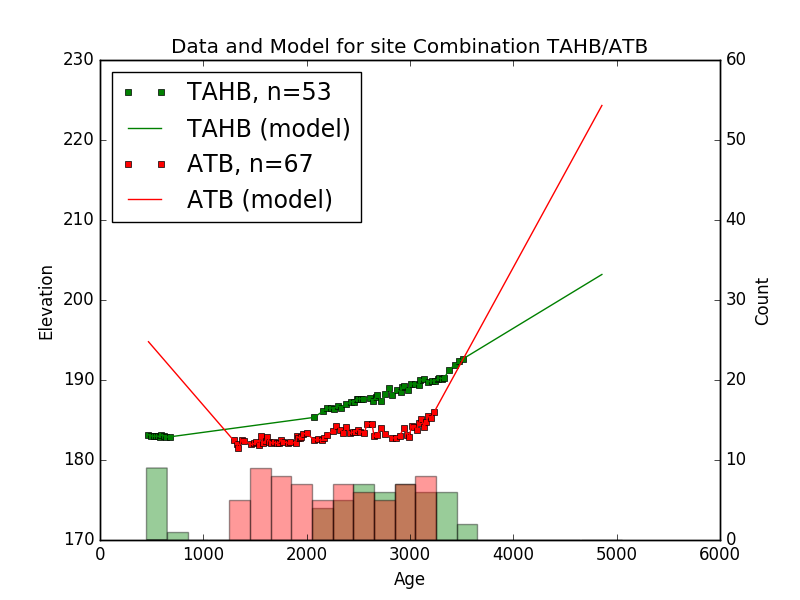
\includegraphics[width=0.72\paperwidth]{data/TAHB-ATB_DataAndModel.png}}
	\caption{TAHB-ATB raw data with linear interpolation model}
	\label{fig:data_TAHBxATB}
\end{figure}

Similar to previous datasets, the combination of TAHB and ATB are constrained to
ages older than
2050 years before present by the Algoma gap, but also have a much shorter range
of age values that
can be considered for GIA calculation, ending at around 3100 years before present.
This is due to TAHB having no data available between 1250-2050 ybp, while ATB
has a great deal of data in this range that can not be considered for this
comparison.
Using only datapoints between 2050 and 3250 years before present results in
relatively poor regressions that are not as well constrained, giving a wide range for
relative GIA of between 19.4-29 cm/century.

\newpage

\begin{figure}[h]
	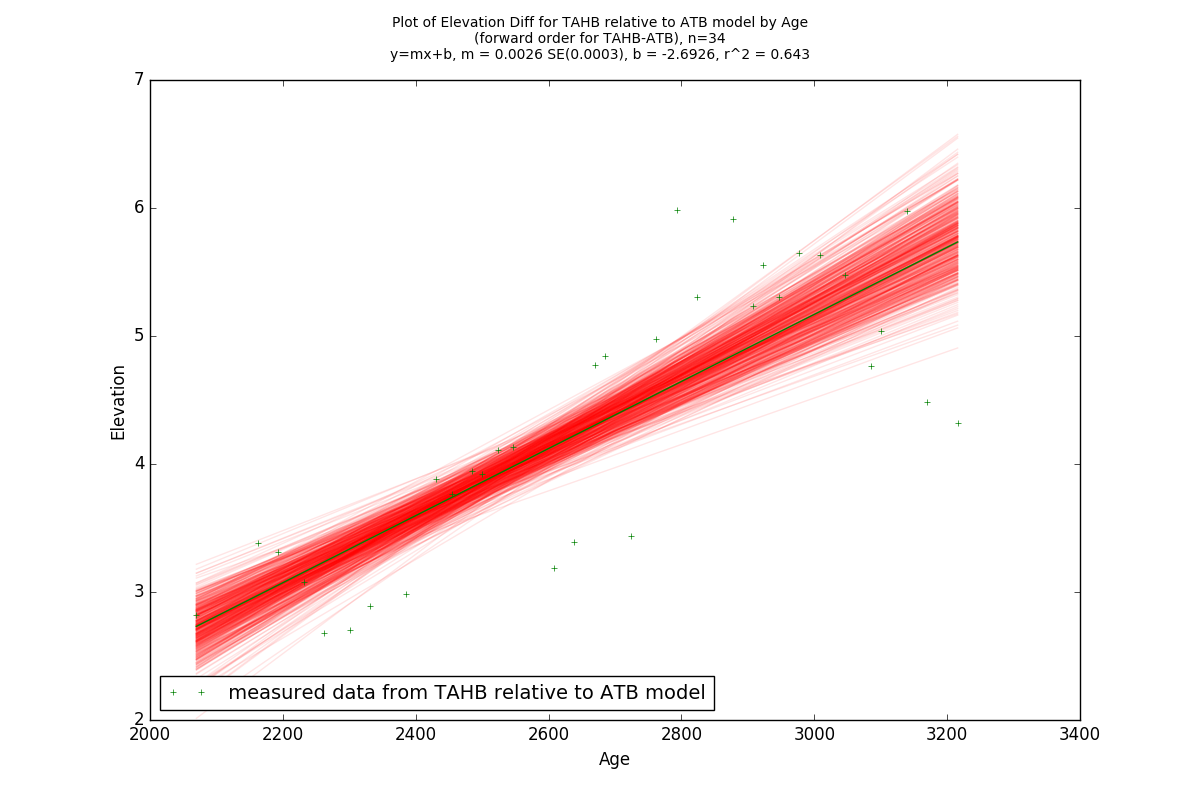
\includegraphics[width=0.9\linewidth]{data/bothNonZero/withinSeventyFivePercent/gias/theGIA_TAHB_relative_to_ATB.png}
	\caption{Differences in elevation measured from the TAHB data to the ATB model}
	\label{fig:gias_TAHBxATB}
\end{figure}
\newpage


\begin{figure}[h]
	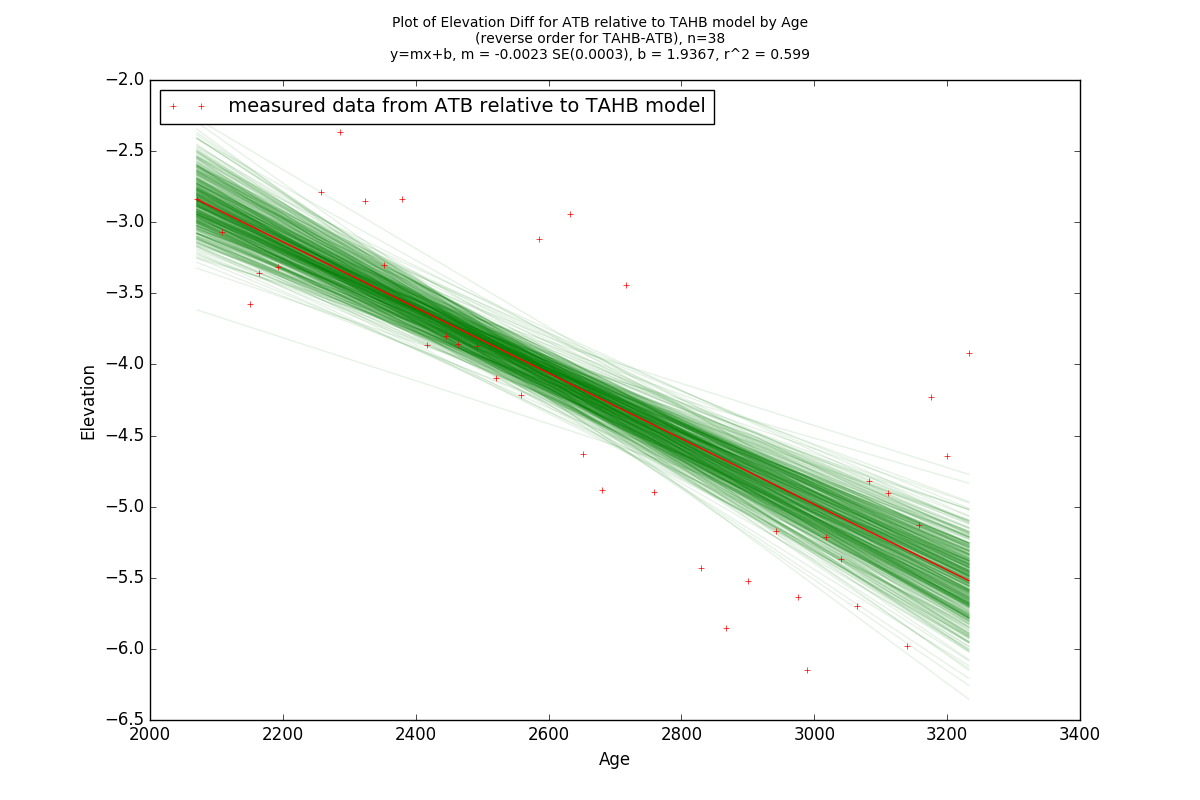
\includegraphics[width=0.9\linewidth]{data/bothNonZero/withinSeventyFivePercent/gias/theGIA_ATB_relative_to_TAHB.png}
	\caption{Differences in elevation measured from the ATB data to the TAHB model}
	\label{fig:gias_ATBxTAHB}
\end{figure}
\newpage






\begin{figure}[h]
	\makebox[\textwidth]{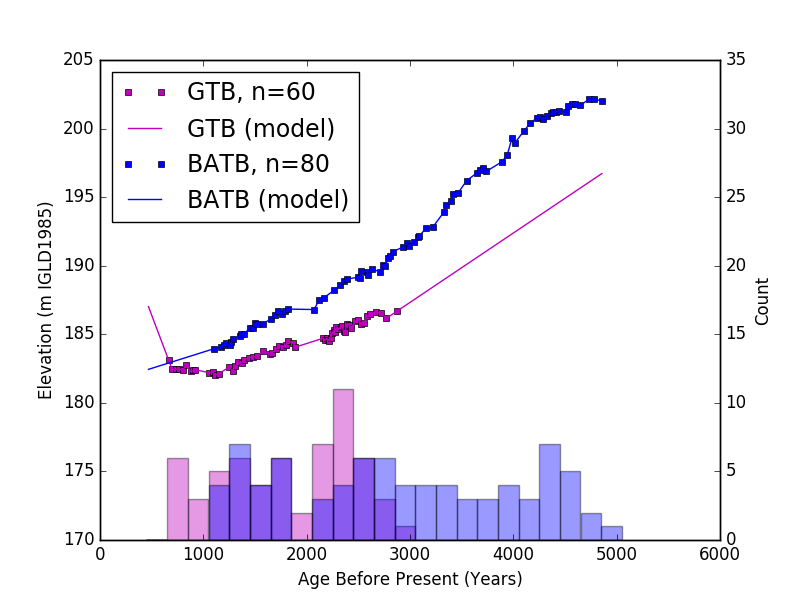
\includegraphics[width=0.72\paperwidth]{data/GTB-BATB_DataAndModel.png}}
	\caption{GTB-BATB raw data with linear interpolation model}
	\label{fig:data_GTBxBATB}
\end{figure}
The GTB BATB combination has a data spread similar to that of ATB \& BATB, with
data available for both datasets from 1050 to 3050 years before present with an
Algoma related gap from 1850 to 2050 years before present. The first case of the
75\% difference cutoff has its first appearance here as the oldest shoreline available from GTB
just falls inside of the 2850-3000 ybp window, causing the entire window to be
used if the only criteria was both dataset counts within that window being non-zero.
The 75\% cutoff prevents this window from being used in this case, as the counts
for the 2850-3000 ybp window differ by 120\%. This rule is useful in identifying
areas of the dataset where both sites have data available, but the density of
one of the datasets in that region is low enough to cause issues with the models
ability to make accurate predictions in between measured datapoints.
The regressions in
Figures \ref{fig:gias_GTBxBATB} \& \ref{fig:gias_BATBxGTB} bear this out,
producing one of the better constrained values at 10.4-12 cm/century.
\newpage

\begin{figure}[h]
	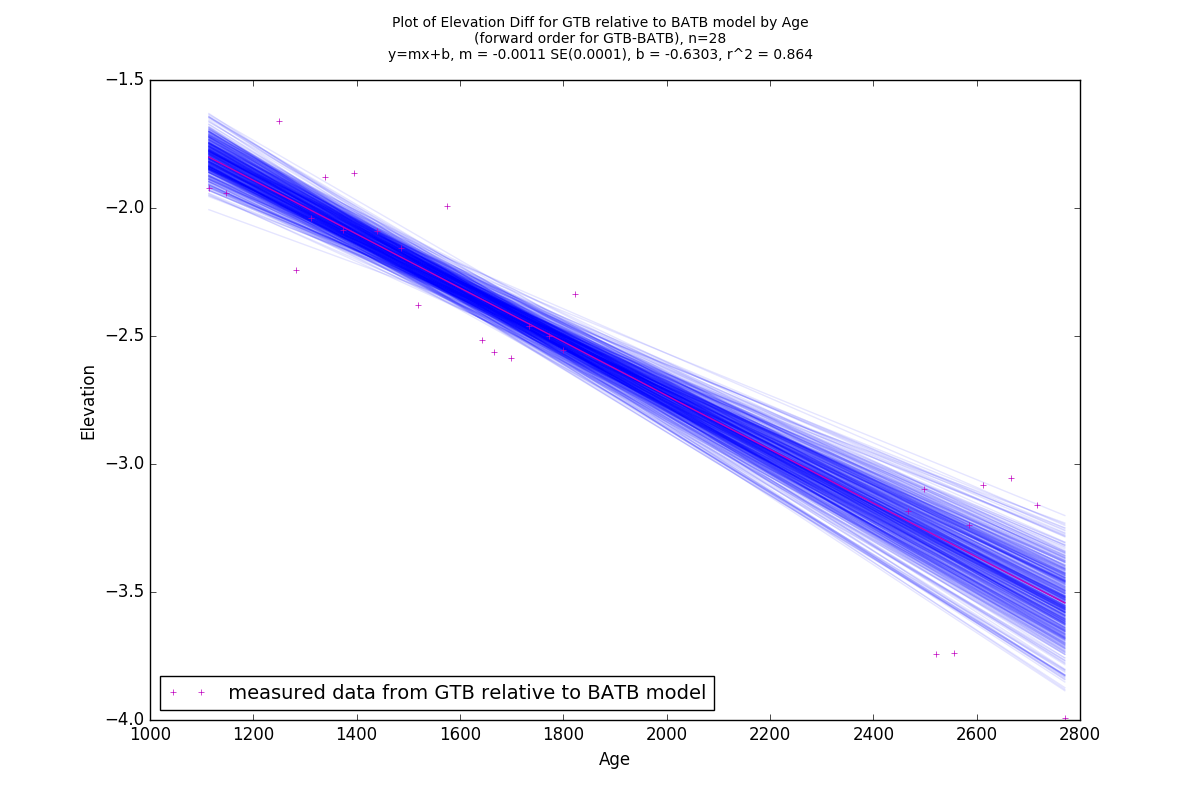
\includegraphics[width=0.9\linewidth]{data/bothNonZero/withinSeventyFivePercent/gias/theGIA_GTB_relative_to_BATB.png}
	\caption{Differences in elevation measured from the GTB data to the BATB model}
	\label{fig:gias_GTBxBATB}
\end{figure}
\newpage


\begin{figure}[h]
	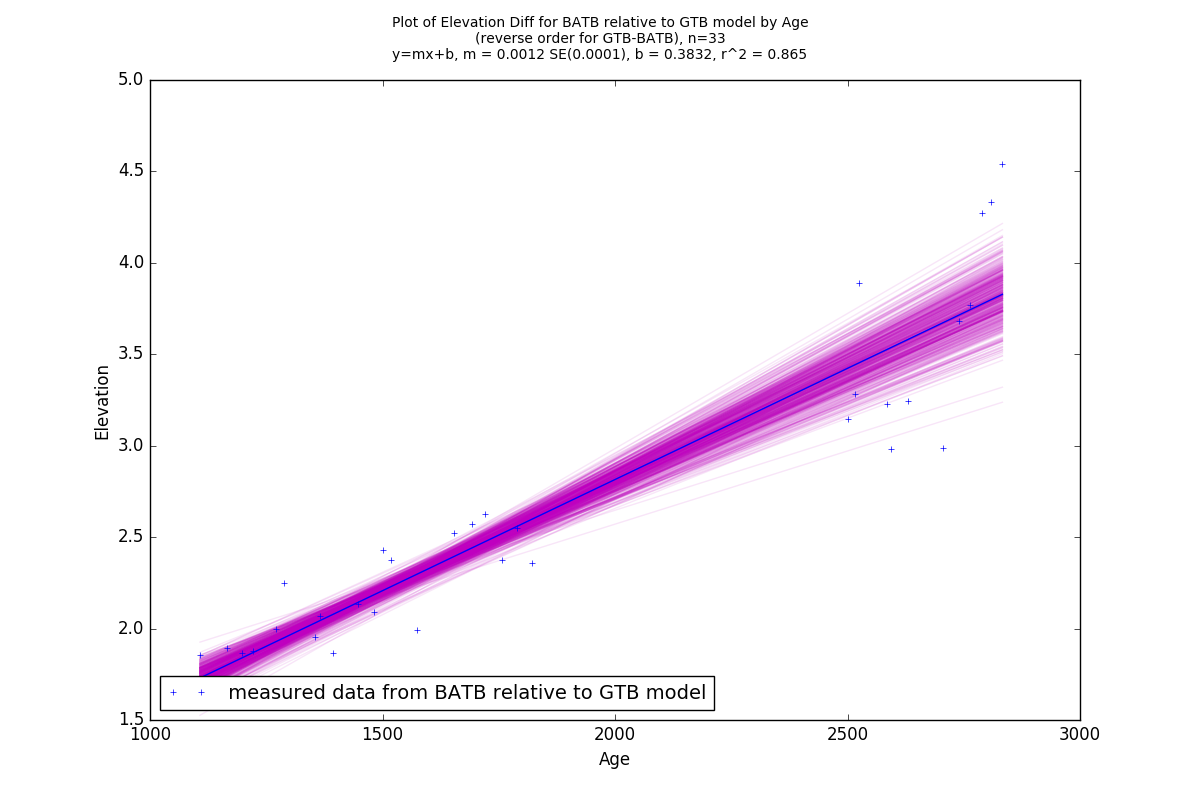
\includegraphics[width=0.9\linewidth]{data/bothNonZero/withinSeventyFivePercent/gias/theGIA_BATB_relative_to_GTB.png}
	\caption{Differences in elevation measured from the BATB data to the GTB model}
	\label{fig:gias_BATBxGTB}
\end{figure}
\newpage









\begin{figure}[h]
	\makebox[\textwidth]{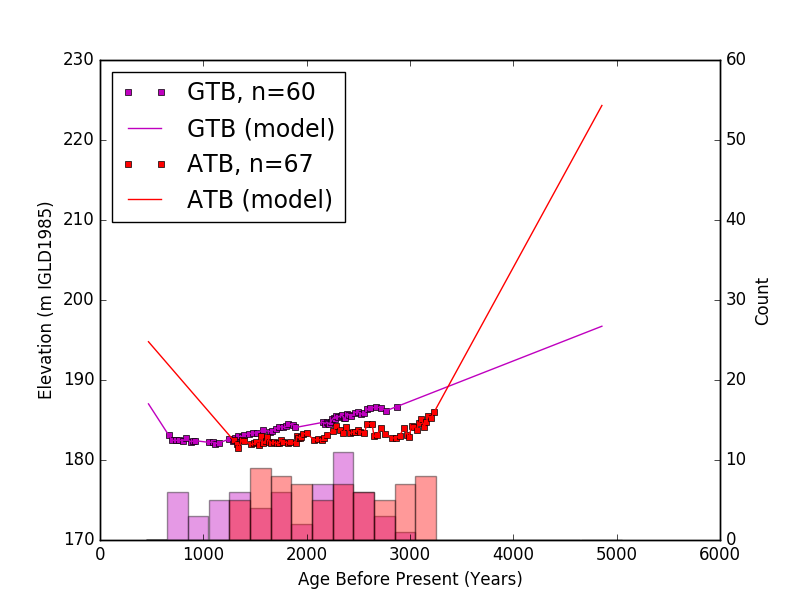
\includegraphics[width=0.72\paperwidth]{data/GTB-ATB_DataAndModel.png}}
	\caption{GTB-ATB raw data with linear interpolation model}
	\label{fig:data_GTBxATB}
\end{figure}

The GTB ATB combination is similar to most of the combinations looked at so far,
windows from 1250 to 3050 ybp containing data for both sites. Two of these windows
fail to qualify for use under the filter due to the site counts differing by more
than 75\%, one from 1850-2050 ybp, and a second one from 2850 to 3050 ybp. Looking
at the graph, it can be seen that both of these windows coincide with ranges of
time where GTB has sparse data, making the GTB models predictions unreliable.
Possibly due to this, the
regressions in Figures \ref{fig:gias_GTBxATB} \& \ref{fig:gias_ATBxGTB} are not
the best constrained constrained, giving a rate of GIA of 9-13.4 cm/century.
\newpage

\begin{figure}[h]
	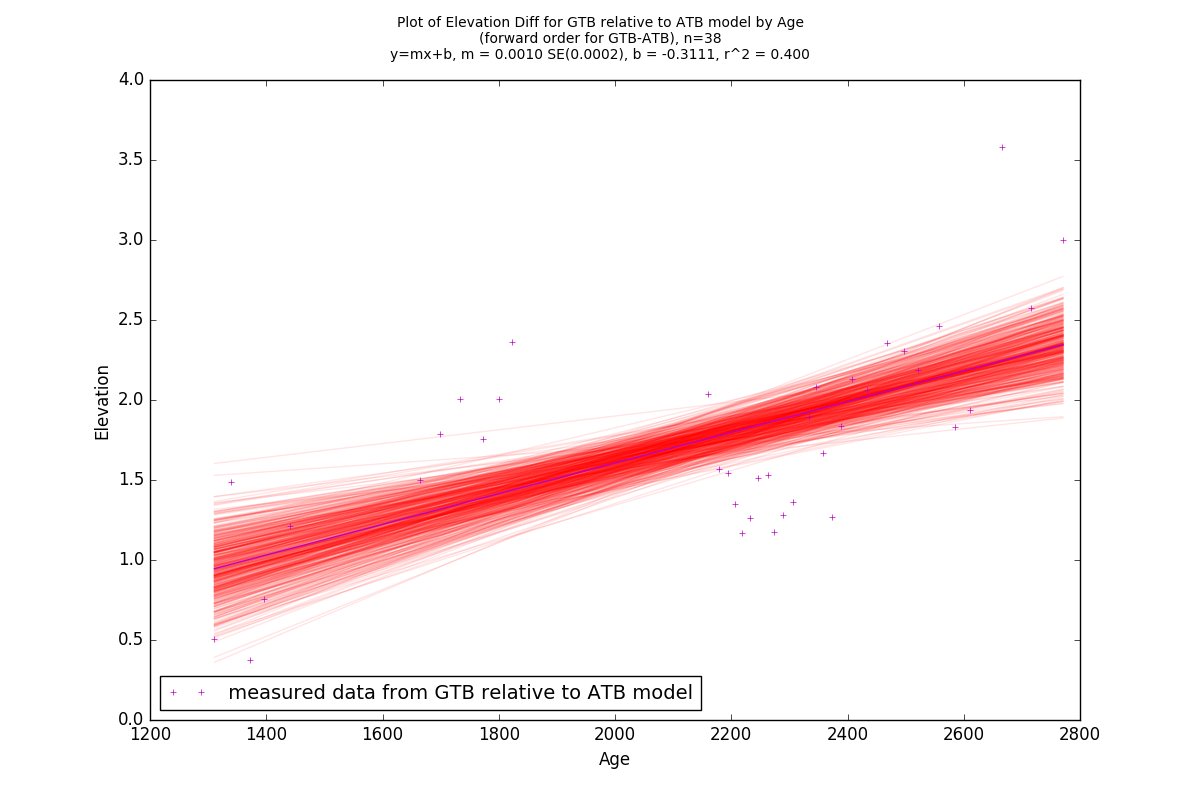
\includegraphics[width=0.9\linewidth]{data/bothNonZero/withinSeventyFivePercent/gias/theGIA_GTB_relative_to_ATB.png}
	\caption{Differences in elevation measured from the GTB data to the ATB model}
	\label{fig:gias_GTBxATB}
\end{figure}
\newpage


\begin{figure}[h]
	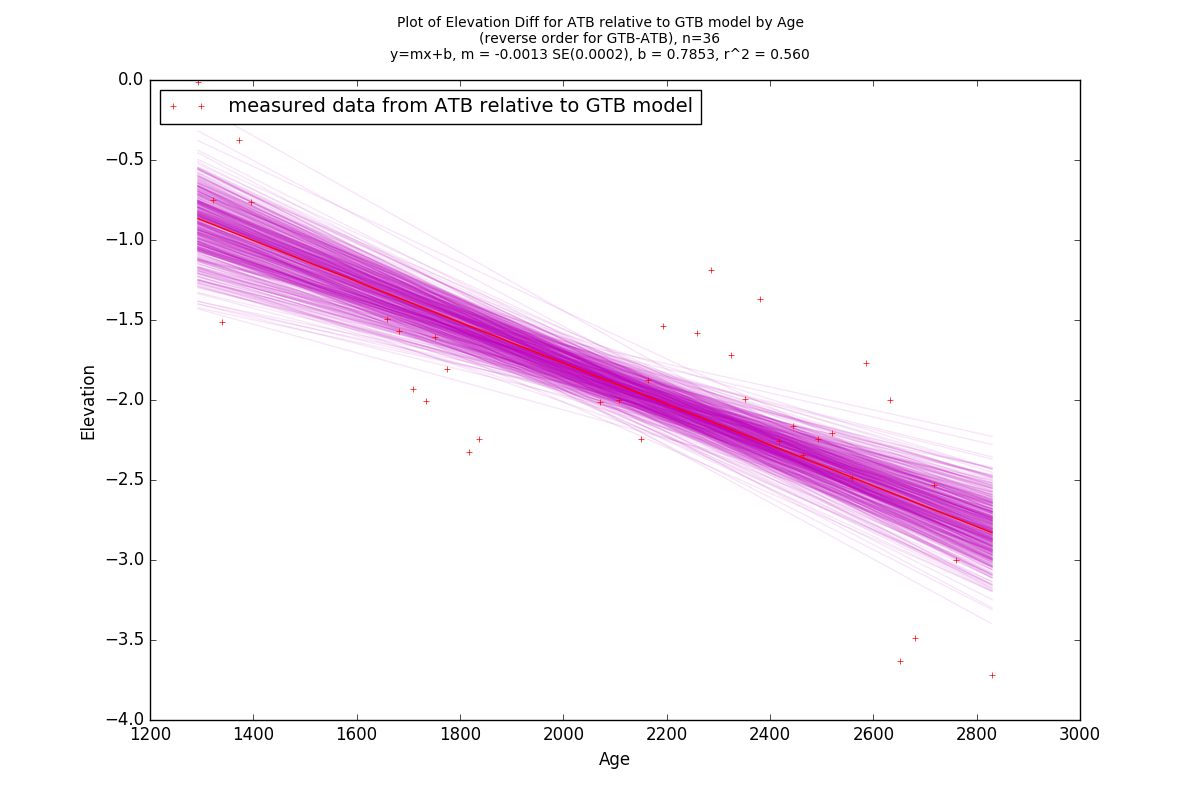
\includegraphics[width=0.9\linewidth]{data/bothNonZero/withinSeventyFivePercent/gias/theGIA_ATB_relative_to_GTB.png}
	\caption{Differences in elevation measured from the ATB data to the GTB model}
	\label{fig:gias_ATBxGTB}
\end{figure}
\newpage










\begin{figure}[h]
	\makebox[\textwidth]{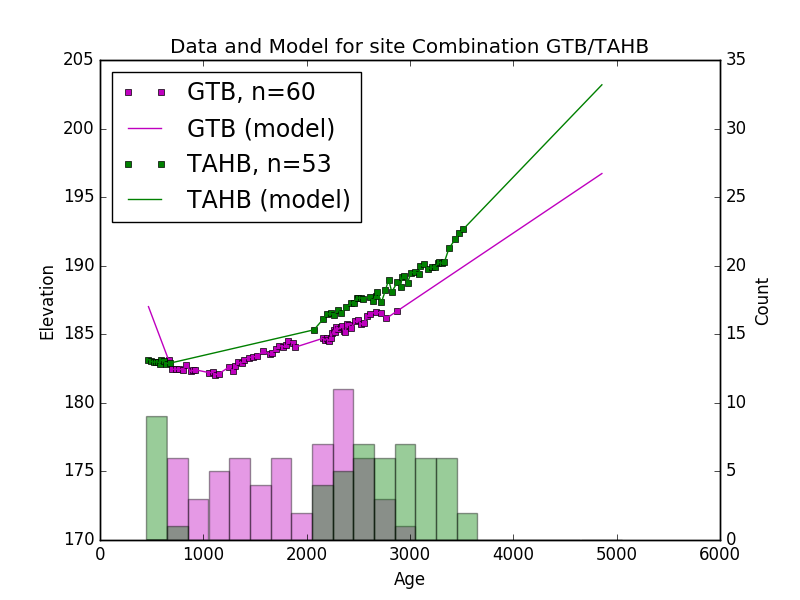
\includegraphics[width=0.72\paperwidth]{data/GTB-TAHB_DataAndModel.png}}
	\caption{GTB-TAHB raw data with linear interpolation model}
	\label{fig:data_GTBxTAHB}
\end{figure}
The final pair of sites GTB and TAHB has by far the most poorly constrained set
of regressions, likely due to the alignment of most of both datasets only giving
sample sizes of n=22 (Figure \ref{fig:gias_TAHBxGTB}) and n=27 (Figure \ref{fig:gias_GTBxTAHB}).
This was due to the valid range of data extending only from 2050 to 2850 ybp. Two
potential windows at 650-850 ybp and 2850-3050 ybp were thrown out due to not
meeting the 75\% rule, as bothwould have produced comparisons between areas of
data in one dataset and a poorly constrained model in the other.
This resulted in an estimate of GIA that ranges anywhere from -2.8-8.6 cm/century,
possibly implying that there may be no difference in vertical adjustment rates
between the TAHB and GTB sites. 
\newpage

\begin{figure}[h]
	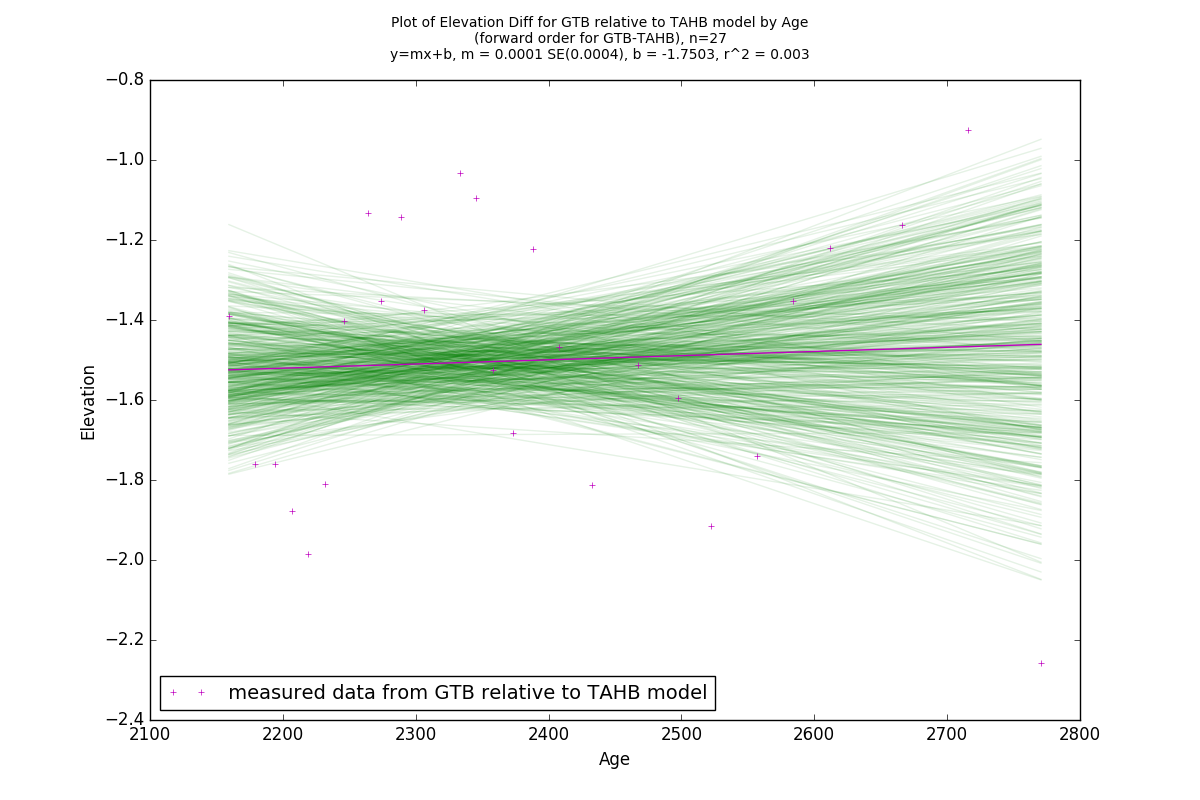
\includegraphics[width=0.9\linewidth]{data/bothNonZero/withinSeventyFivePercent/gias/theGIA_GTB_relative_to_TAHB.png}
	\caption{Differences in elevation measured from the GTB data to the TAHB model}
	\label{fig:gias_GTBxTAHB}
\end{figure}
\newpage


\begin{figure}[h]
	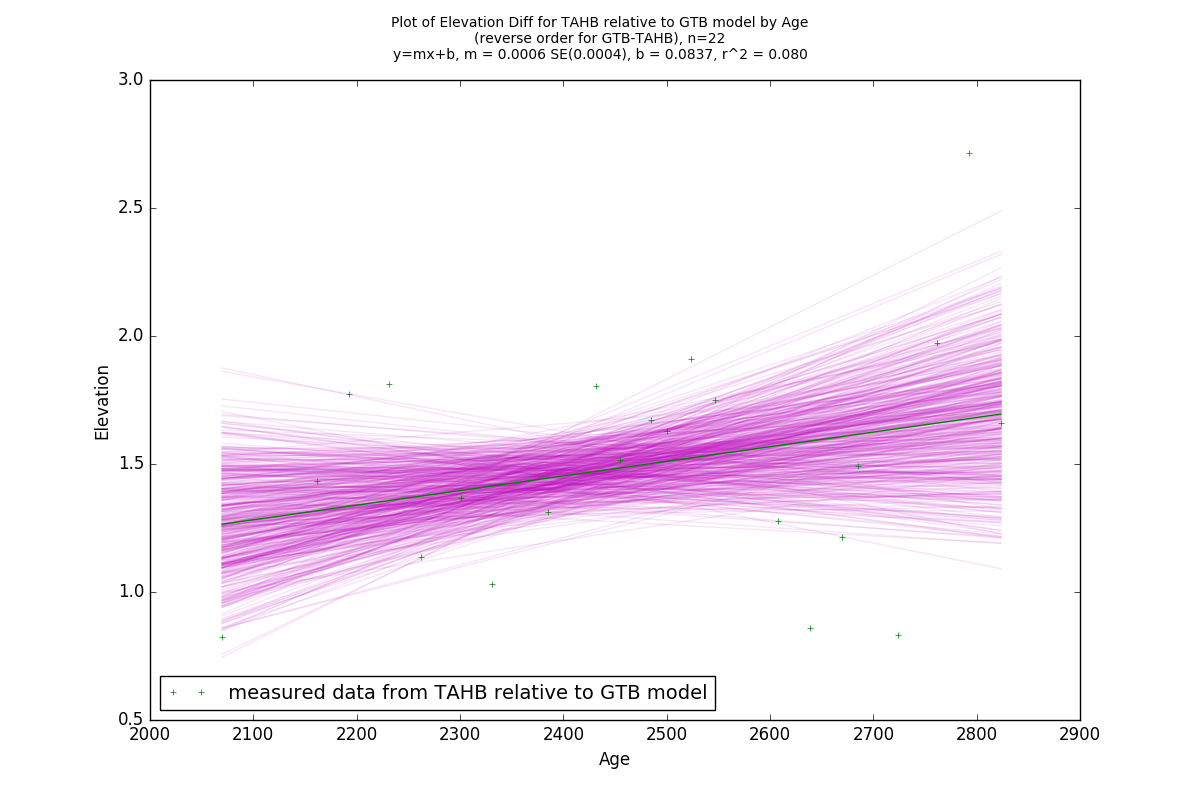
\includegraphics[width=0.9\linewidth]{data/bothNonZero/withinSeventyFivePercent/gias/theGIA_TAHB_relative_to_GTB.png}
	\caption{Differences in elevation measured from the TAHB data to the GTB model}
	\label{fig:gias_TAHBxGTB}
\end{figure}
\newpage


\begin{figure}[h]
	\makebox[\textwidth]{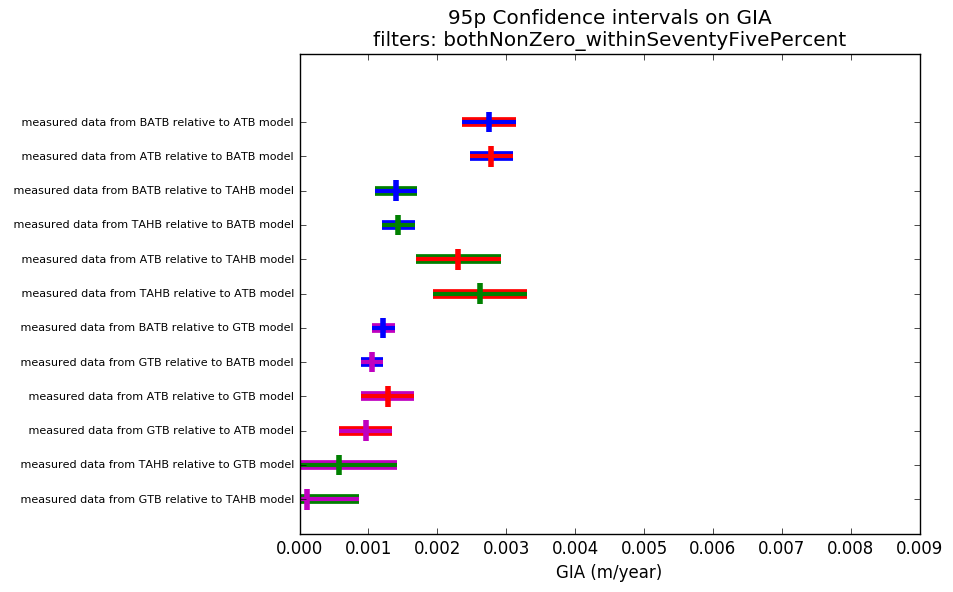
\includegraphics[width=0.6\paperwidth]{data/bothNonZero/withinSeventyFivePercent/gias/intervals.png}}
	\caption{95p Confidence intervals on GIA rates obtained from site comparisons}
	\label{fig:intervalsGIA}
\end{figure}


\newpage

